\section {Radosław Myśliwiec}

Zasada indukcji matematycznej:
$$ (P(0) \land (\forall_{n \in \mathbb{N}} : P(n) \Rightarrow P(n_{++}))) 
\Rightarrow \forall_{n \in \mathbb{N}} : P(n) $$

\begin{figure} [htpb]
    \centering
    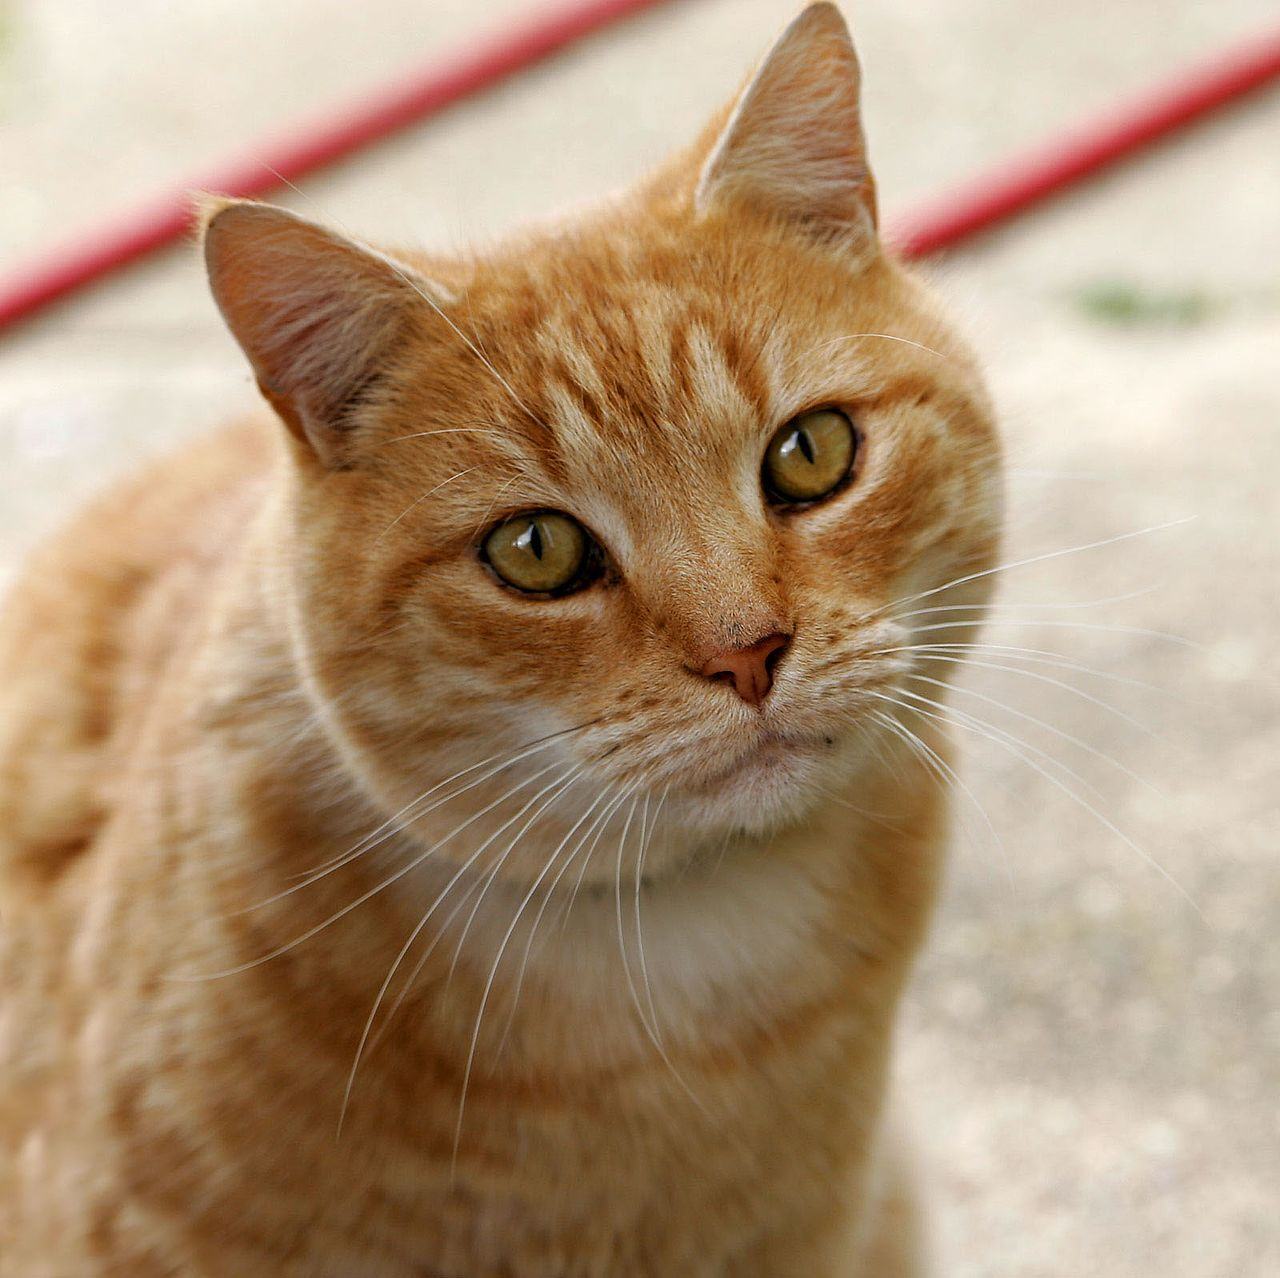
\includegraphics[width=200px]{pictures/cat.jpg}
    \caption{Kotek}
    \label{kot}
\end{figure}

\begin{table}[htbp]
\centering
\begin{tabular}{|l|l|l|l|l|}
\hline
a & b & c & d & e \\ \hline
f & g & h & i & j \\ \hline
\end{tabular}
\caption{Tabela}
\label{tab:5_tabela}
\end{table}

\begin{itemize}
    \item Ala
    \item ma
    \item kota
    \item rudego (Figure: \ref{kot})
\end{itemize}

\begin{enumerate}
    \item Kot
    \item ma
    \item Ale
\end{enumerate}

\emph{Police} are a constituted body of persons empowered by a state, with the aim 
to enforce the law, to ensure the safety, health and possessions of citizens, 
and to prevent crime and civil disorder.

Their lawful powers include arrest and the use of force legitimized by the 
state via the monopoly on violence. The term is (Cat picture on page: \pageref{kot}) 
most commonly associated with 
\underline{the police} forces of a sovereign state that are authorized to exercise the police 
power of that state within a defined legal or territorial area of responsibility. 

\textbf{Police} forces are often defined as being separate from the military and 
other organizations (Look table \ref{tab:5_tabela}) involved in the defense of the 
state against foreign 
aggressors; however, gendarmerie are military units charged with civil policing. 
Police forces are usually public sector services, funded through taxes.
